%%                             -*- Mode: Latex -*- 
%% refman.tex --- Seed Reference Manual
%% Author          : Marcel Turcotte
%% Created On      : Tue Jul 12 10:26:00 2005
%% Last Modified By: Marcel Turcotte
%% Last Modified On: Fri Aug  5 16:30:56 2005
%%
%% This copyrighted source code is freely distributed under the terms
%% of the GNU General Public License. 
%% See the files COPYRIGHT and LICENSE for details.

%% Coding convention:
%% - use texttt for directories, options and commands

\documentclass{article}

\title{Seed 1.0: RNA Secondary Structure Motif Inference}

\author{Truong Nguyen and Marcel Turcotte}

\date{Copyright \copyright\ 2003-05 University of Ottawa}

\usepackage[margin=1in]{geometry}

\usepackage{graphicx}
\graphicspath{{figs/}}

\begin{document}

\maketitle

\begin{abstract}

Seed is a novel approach for discovering consensus secondary structure
motifs in a set of unaligned RNA sequences\cite{Nguyen2005}. Its representation of
secondary structure motifs combine sequence and structure
information. State-of-the-art data structures, suffix arrays in
particular, are used to enumerate exhaustively the space of possible
motifs. Suffix arrays (SAs) are used for two purposes. First, to
enumerate efficiently stem structures, including internal
loops. Second, SAs are used to match secondary structure
expressions. This document serves as a reference manual and it also
attempts to give you indications to help you control the runtime of
the program.

\end{abstract}

\section{Installing}

Seed is written in ISO C and uses some of extensions of the standard
ISO C99 (use the option \texttt{-std=c99} with GCC).  The software
system and its libraries are known to run on Linux (RedHat 9 and
Fedora Core 3)/i386 (Makefile.gcc), Solaris 9/Sparc (Makefile.sparc)
and Solaris 9/i386 (Makefile.i386). Select the appropriate Makefile
for your system, either copy this file to \texttt{Makefile} or use
\texttt{make -f Makefile.arch}.

\subsection{LIBRNA (Optional)}

Seed makes use of LIBRNA from the Vienna RNA Package to calculate and
report the free energy of matching sequences.  In order to enable this
feature, you need to install the package first (follow the
instructions therein).  Locate and edit the following section of the Makefile,
\begin{verbatim}
RNALIB =
RNALIB_INCLUDE =
RNALIB_LIB =
RNALIB_LIBS =
\end{verbatim}
You will need to add the following declaration \texttt{-DRNALIB} to
\texttt{RNALIB} so that the C preprocessor includes the sections for
LIBRNA into the compilation.  You will also need to give the path to
the include and library directories.  Here is a template that we use
for our local Linux/i386 installation.
\begin{verbatim}
RNALIB = -DRNALIB
RNALIB_INCLUDE = -I/local/bio/sfw/include
RNALIB_LIB = -L /local/bio/sfw/exec/i386-pc-linux-gnu/lib/
RNALIB_LIBS = -lRNA -lm
\end{verbatim}

\subsection{Seed}

The compilation and installation of Seed is a straight forward
process.  Type \texttt{make}, possibly \texttt{make check} and then
\texttt{make install}.  The default option is to install Seed into the
\texttt{bin} subdirectory of the distribution top directory. This
option is controled by the variable \texttt{BINDIR} of the
main Makefile.  By default, Seed is statistically linked and does not
require any external files, therefore, is can safely been moved to any
location (simply make sure that this directory is found on your
\texttt{PATH}).

\section{Basic usage}

Typing \texttt{seed}, \texttt{seed -h} or \texttt{seed --help} lists
all the valid options.
\begin{verbatim}
> seed

Usage: seed [options] file
where file is a FASTA file that contains k input RNA sequences.
                                                                                                    
Options:
     --seed <n>                (default 0)
     --stem_min_len <n>        (default 3)
     --stem_max_gu <n>         (default 100)
     --min_num_stem <n>        (default 1)
     --max_num_stem <n>        (default 2)
     --stem_max_separation <n> (default 150)
     --skip_keep_longest_stems (default false)
     --loop_min_len <n>        (default 4)
     --nogu                    (default false)
     --range <n>               (default 1)
     --max_mismatch <n>        (default 2)
     --max_fixed_pos <n>       (default 100)
     --min_base_pair <n>       (default 5)
     --min_support <n>         (default 0.70)
  -t --time_limit <n>          (default 0)
     --save_all_matches        (default false)
     --save_as_ct              (default false)
     --save_motifs             (default false)
  -m --match_file <file>       (no default)
  -d --destination <dir>       (default .)
  -p --print_level <n>         (default 1)
  -q --quiet                   (default false)
  -v --version
  -h --help
\end{verbatim}                                                                                                    

The minimum requirement is an input FASTA file containing $k$ input RNA
sequences.
\begin{verbatim}
> seed examples/tRNAs-2.fas

Seed 1.0 [Jul 23 2005] - RNA secondary structure motif inference
                                                                                                    
Copyright (C) 2003-05 University of Ottawa
All Rights Reserved
                                                                                                    
This program is distributed under the terms of the
GNU General Public License. See the source code
for details.
                                                                                                    
[ find_all_stems ]
[ size of the motif list is 164 ]
[ filter_by_support ]
[ size of the motif list is 146 ]
[ filter_keep_longest_stems ]
[ size of the motif list is 89 ]
[ fix_all ]
[ size of the motif list is 391 ]
[ combine_all ]
[ generating all 2 stems motifs ]
[ size of the motif list is 391 ]
[ done ]
[ size of the motif list is 958 ]
[ postprocess ]
[ size of the motif list is 958 ]
[ elapsed time 2 minutes, 34 seconds ]
[ total number of match operations is 221004 ]
\end{verbatim}
By default, the first sequence (index 0) is used as the seed.  The
program will first enumerate all the possible stems that are at least
three nucleotides long, allowing for GU base pairs and up to one
mismatch. This list is filtered to preserve only the motifs that are
present in 70\% of the input sequences.  The algorithm then creates
new motifs, first making the generic stems specific by adding
base pairs from the seed sequence. Secondly, the algorithm combines
the one-stem motifs together to produce two-stem motifs.  By default,
Seed stops this process at two stems.  It reports statistics and then
stop. No motifs are saved by default, this allows you to explore the
effect of various options and avoid unfortunate suprises, such as
writing out 250 Mbytes of data.

Once a suitable set of options has been found, use one of the many
options for saving the results.  Here is a possible scenario.
\begin{verbatim}
> mkdir results/01
> seed --quiet --destination results/01 --save_motifs --min_num_stem 3 \ 
  --max_num_stem 100 --range 2 examples/tRNAs-2.fas
\end{verbatim}
The motifs will be saved (in XML format) in files named
\texttt{motif.xml} located into subdirectories of the destination
folder.  The destination folder also contains a file named
\texttt{params.xml} that records the options that were used for this
run.

\section{Options}

\begin{description}
\item[\texttt{--seed <n>} (default 0):] This option selects a specific
  seed sequence. Valid values are integers in the range $0 \ldots
  k-1$, where $k$ is the number of input sequences.
\item[\texttt{--stem\_min\_len <n>} (default 3):] During the first step
  of the search, Seed enumerates all the valid stems.  For a given
  pair of positions $i$ and $j$, Seed computes the longest
  extension $l$ such that $S[i,i+l-1]$ and $S[j, j-l+1]$ forms a
  canonical stem (a stem made of canonical base pairs only, possibly
  including GU base pairs), if the current number of
  mismatches is smaller than the user defined threshold then Seed
  repeats this process from $i+l+1$ and $j-l-1$.  This option controls
  the minum value of $l$ for each iteration of the extension process.
\item[\texttt{--stem\_max\_gu <n>} (default 100):] Controls the
  maximum number of GU base pairs.
\item[\texttt{--min\_num\_stem <n>} (default 1):] Motifs having less
  than this number of stems are not reported.
\item[\texttt{--max\_num\_stem <n>} (default 2):] Stops the algorithm
  when all the motifs having this many stems have been produced.
\item[\texttt{--stem\_max\_separation <n>} (default 150):]  In the stem
  enumeration step, limits the maximum distance between the start and
  end of a stem.
\item[\texttt{--skip\_keep\_longest\_stems} (default false):]
  Generates all the stems from \texttt{stem\_min\_len} up to the
  maximum possible size.
\item[\texttt{--loop\_min\_len <n>} (default 4):] Defines the minimum
  size of loops.
\item[\texttt{--nogu} (default false):] Disallow GU base pairs.
\item[\texttt{--range <n>} (default 1):] The number of additional base
  pairs that are allowed when matching a range element (when
  calculating the support of a motif).
\item[\texttt{--max\_mismatch <n>} (default 2):] The maximum number of
  mismatches that are allowed when enumerating stems and matching motifs.
\item[\texttt{--max\_fixed\_pos <n>} (default 100):] The maximum
  number of
  base pairs that will be fixed in fix\_all stem.
\item[\texttt{--min\_base\_pair <n>} (default 5):] The minum number of
  base pairs for the sum of all base pairs.
\item[\texttt{--min\_support <n>} (default 0.70):] The fraction of the
  input sequences that a motif matches to be retained.
\item[\texttt{-t --time\_limit <n>} (default 0):] Limits the execution time
  to the specified number of minutes.
\item[\texttt{--save\_all\_matches} (default false):] Simple motifs
  may match the input sequences at several locations, with this option
  all of them will be saved.
\item[\texttt{--save\_as\_ct} (default false):] Saves the matches as
  ct (MFOLD) files. This can be convenient to visualise, compare and
  cluster the results.
\item[\texttt{--save\_motifs} (default false):] Save the motifs as XML
  files, creates a directory structure with one directory per motif.
\item[\texttt{-d --destination <dir>} (default .):] Where to save the motifs.
\item[\texttt{-m --match\_file <file>} (no default):] Saves all the
  matches into a single file.
\item[\texttt{-p --print\_level <n>} (default 1):] Increases/decreases
  the verbosity.
\item[\texttt{-q --quiet} (default false):] Turns off all the traces.
\item[\texttt{-v --version}:] Prints the version information.
\item[\texttt{-h --help}:] Lists all the options.
\end{description}

\section{Controlling the size of the search space}

Seed performs a breath-first-search of the secondary structure motif space
induced from a seed sequence.  Seed provides many options to control
the size of the search space, which can be quite large.  A good
understanding of the motif discovery algorithm, its parameters and the
problem to solve will help reduce the execution time.

Seed searches a space of secondary structure motif induced from a
seed sequence.  Selecting a shorter input sequence as the seed will greatly
reduce the size of the initial list of motifs and, consequently,
greatly reduce the execution time. This leads to a more general
observation, reducing the size of the initial list of motifs reduces
the branching factor of the search tree, and will also greatly reduce
the execution time. Other ways to reduce the size of the initial list
of motifs include: specifying a small number of fixed positions
(\texttt{--max\_fixed\_pos 0} produces generic motifs).  Limiting the
maximum separation between elements of a base pair diminishes the size
of the initial list of motif (\texttt{--stem\_max\_separation 30} will
produce motifs such that the maximum distance between any two elements
of a pair is 30 nucleotides or less). Requiring a higher level of
support is also an effective way to keep the size of the open list of
motifs short.

When everything else fails, imposing a time limit will allow you to
obtain some results that hopefully will help you defining new
constraints to further reduce the search space.  Seed uses an iterative
deepening algorithm for enumerating the motifs, it will first
enumerate all the one-stem, two-stem motifs, and so on.  Using a time
constraint allows you to explore the search tree up to a certain depth.

% \section{Source code and data structures}
% 
% \begin{figure}\centering
% 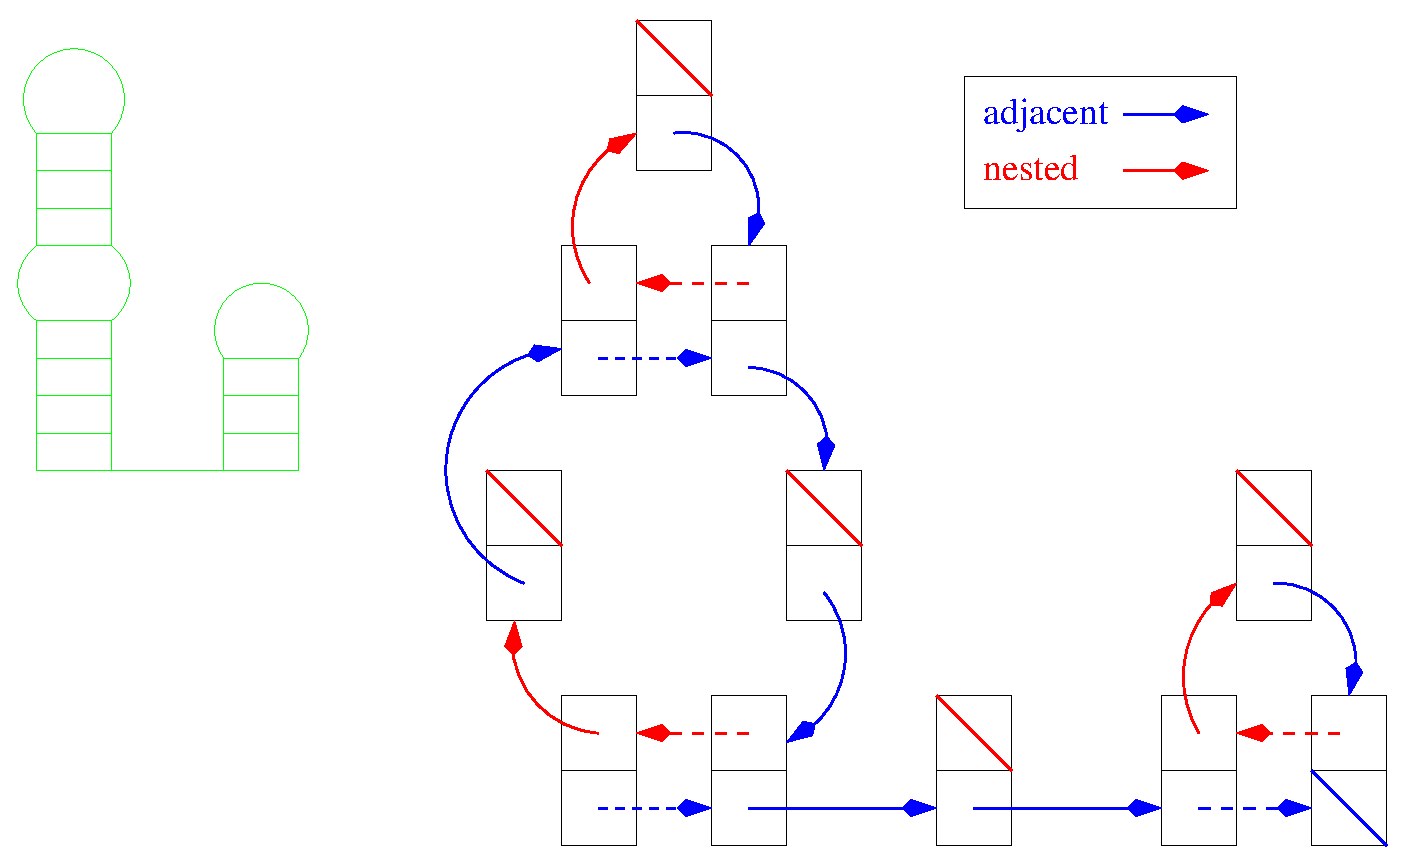
\includegraphics[width=\textwidth]{rna_expression}
% \caption{}\label{fig:expression}
% \end{figure}


\newpage

\bibliographystyle{plain}
\bibliography{seed}

\end{document}
